

\section{Closing Plots (Filling the Area Under Plots)}
\begin{command}{\closedcycle}
	Provide |\closedcycle| as \meta{trailing path commands} after |\addplot| to draw a closed line from the last plot coordinate to the first one.
	
	Use |\closedcycle| whenever you intend to fill the area under a plot.

\begin{codeexample}[]
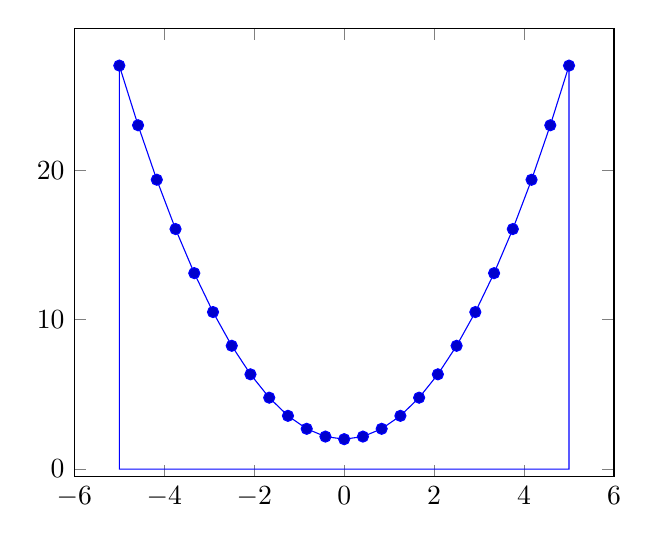
\begin{tikzpicture}
	\begin{axis}
	\addplot {x^2+2} \closedcycle;
	\end{axis}
\end{tikzpicture}
\end{codeexample}

\begin{codeexample}[]
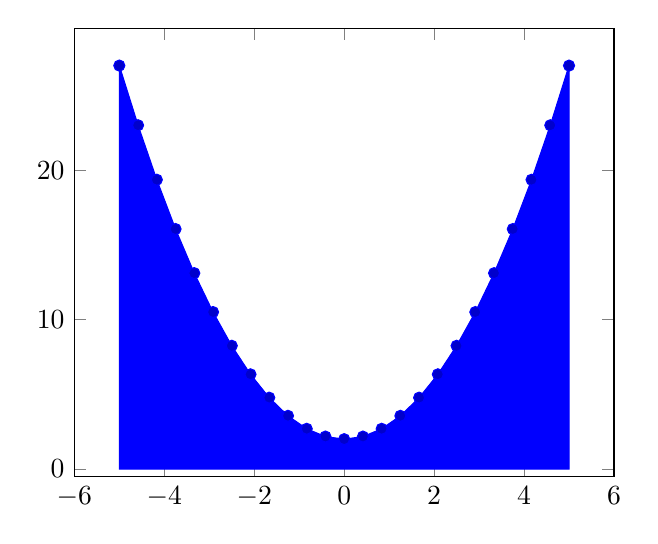
\begin{tikzpicture}
	\begin{axis}
	\addplot+[fill] {x^2+2} \closedcycle;
	\end{axis}
\end{tikzpicture}
\end{codeexample}
	In case of stacked plots, |\closedcycle| connects the current plot with the previous plot instead of connecting with the $x$~axis\footnote{The implementation for stacked plots requires some additional logic to determine the filled area: \lstinline{\\closedcycle} will produce a \texttt{plot coordinates} command with \emph{reversed} coordinates of the previous plot. This is usually irrelevant for end users, but it assumes that the plot's type is symmetric. Since constant plots are inherently asymmetric, \lstinline{\\closedcycle} will use \texttt{const plot mark right} as reversed sequence for \texttt{const plot mark left}.}.
\begin{codeexample}[]
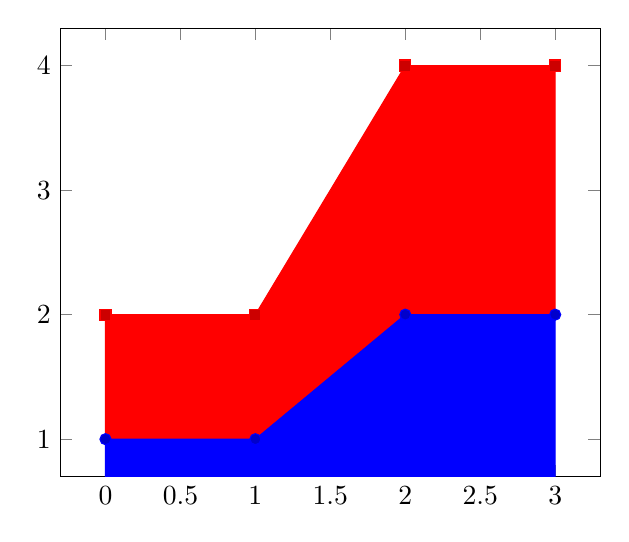
\begin{tikzpicture}
	\begin{axis}[stack plots=y]
	\addplot+[fill] coordinates 
		{(0,1) (1,1) (2,2) (3,2)} \closedcycle;
	\addplot+[fill] coordinates 
		{(0,1) (1,1) (2,2) (3,2)} \closedcycle;
	\end{axis}
\end{tikzpicture}
\end{codeexample}
\end{command}

Closing a plot is also possible for three--dimensional axes:
\begin{codeexample}[]
\begin{tikzpicture}
\pgfplotstableread{
plot1     plot2     plot3     plot4
0.0045    0.0029    0.0089    0.0001
0.0040    0.0028    0.0083    0.0009
0.0035    0.0027    0.0073    0.0014
0.0029    0.0025    0.0062    0.0016
0.0024    0.0023    0.0050    0.0016
0.0019    0.0020    0.0038    0.0013
0.0014    0.0017    0.0027    0.0010
0.0010    0.0015    0.0018    0.0006
0.0007    0.0012    0.0010    0.0001
0.0004    0.0009    0.0005   -0.0004
0.0002    0.0007    0.0001   -0.0008
0.0001    0.0005   -0.0000   -0.0012
0.0000    0.0004   -0.0000   -0.0015
0.0000    0.0003    0.0001   -0.0018
0.0000    0.0002    0.0002   -0.0019
0.0001    0.0001    0.0005   -0.0021
0.0001    0.0001    0.0007   -0.0021
0.0002    0.0001    0.0009   -0.0021
0.0002    0.0000    0.0012   -0.0021
0.0002    0.0000    0.0013   -0.0021
0.0003    0.0000    0.0015   -0.0020
0.0003    0.0001    0.0016   -0.0020
0.0003    0.0001    0.0017   -0.0019
0.0003    0.0001    0.0017   -0.0018
0.0003    0.0001    0.0017   -0.0018
0.0003    0.0001    0.0017   -0.0017
0.0003    0.0001    0.0017   -0.0016
0.0003    0.0001    0.0017   -0.0016
0.0003    0.0001    0.0016   -0.0015
0.0003    0.0001    0.0016   -0.0015
0.0003    0.0001    0.0016   -0.0014
0.0003    0.0001    0.0016   -0.0014
0.0003    0.0001    0.0016   -0.0013
0.0003    0.0002    0.0015   -0.0013
0.0003    0.0002    0.0015   -0.0013
0.0003    0.0002    0.0015   -0.0012
0.0003    0.0002    0.0015   -0.0012
0.0003    0.0002    0.0015   -0.0011
0.0003    0.0002    0.0015   -0.0011
0.0003    0.0002    0.0014   -0.0010
}\tabledata
\begin{axis}[
    zmin=-0.001,
    area plot/.style={
        fill opacity=0.75,
        draw=orange!80!black,thick,
        fill=orange,
        mark=none,
    },
	ytick={1,...,4},
	yticklabel=plot\pgfmathprintnumber{\tick},
]
\pgfplotsinvokeforeach{4,3,...,1}{
    \addplot3 [area plot] table [x expr=\coordindex, y expr=#1, z=plot#1]
      {\tabledata} \closedcycle;
}
\end{axis}
\end{tikzpicture}
\end{codeexample}

Note that |\closedcycle| has been designed for functions (i.e.\ for a plot where every $x$ has at most one $y$ value). For arbitrary curves, you can safely use the \tikzname\ path \declareandlabel{--cycle} instead which simply connects the last and the first path element:
\begin{codeexample}[]
\begin{tikzpicture}
	\begin{axis}
	\addplot coordinates 
		{(0,1) (1,2) (0,3) (-1,2)};
	\end{axis}
\end{tikzpicture}
\end{codeexample}

\begin{codeexample}[]
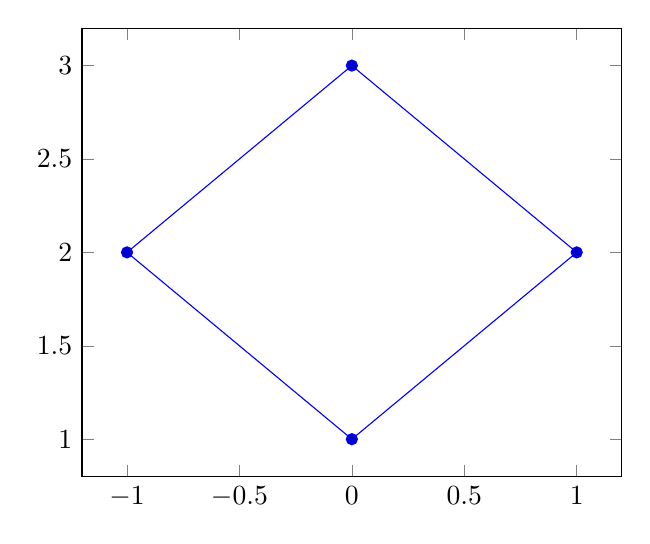
\begin{tikzpicture}
	\begin{axis}
	\addplot coordinates 
		{(0,1) (1,2) (0,3) (-1,2)} --cycle;
	\end{axis}
\end{tikzpicture}
\end{codeexample}

\begin{codeexample}[]
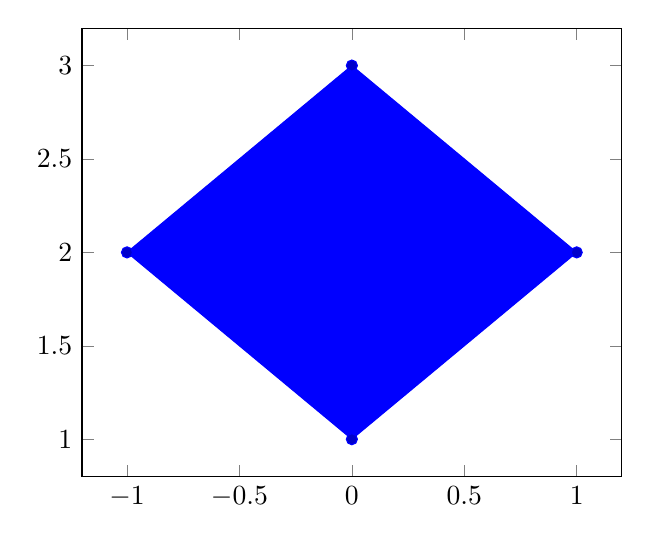
\begin{tikzpicture}
	\begin{axis}
	\addplot+[fill] coordinates 
		{(0,1) (1,2) (0,3) (-1,2)} --cycle;
	\end{axis}
\end{tikzpicture}
\end{codeexample}
The |--cycle| is actually a path instruction of \cite{tikz}; it connects the first and the last coordinate of one path. Note that this is automatically done for |fill|ed paths.
